\documentclass[12pt]{article}
\usepackage[catalan]{babel}
\usepackage[utf8]{inputenc}
\usepackage{listings}
\usepackage{color}
\usepackage{graphicx}
\usepackage{verbatim}
\usepackage[obeyspaces]{url}
\usepackage{appendix}
\usepackage{dirtytalk}

\definecolor{codegreen}{rgb}{0,0.6,0}
\definecolor{codegray}{rgb}{0.5,0.5,0.5}
\definecolor{codepurple}{rgb}{0.58,0,0.82}
\definecolor{backcolour}{rgb}{0.95,0.95,0.92}
 
\lstset{
	backgroundcolor=\color{backcolour},   
	breaklines=true, 
	numbers=left,
	basicstyle=\footnotesize,
	backgroundcolor=\color{backcolour},   
    commentstyle=\color{codegreen},
    keywordstyle=\color{magenta},
    numberstyle=\tiny\color{codegray},
    stringstyle=\color{codepurple},
    basicstyle=\footnotesize,
    breakatwhitespace=false,         
    breaklines=true,                 
    captionpos=b,                    
    keepspaces=true,                 
    numbers=left,                    
    numbersep=5pt,                  
    showspaces=false,                
    showstringspaces=false,
    showtabs=false,                  
    tabsize=2
}
\setlength{\parindent}{0pt}

\begin{document}
\begin{titlepage}
		\centering
		
\includegraphics[width=0.5\textwidth]{imatges/logo.png}\par\vspace{1cm}
		{\huge\bfseries Projecte final\par}
		\vspace{1cm}
		{\scshape\Large Màster en enginyeria informàtica\par}
		\vspace{1.5cm}
		{\Large\itshape Oscar Galera i Alfaro\par}
		\vspace{1cm}
		{\Large\itshape Mineria de dades\par}
		\vspace{2cm}
		\vfill
		\vfill
		{\large \today\par}
\end{titlepage}
\clearpage
\tableofcontents
\clearpage
\listoffigures


\clearpage
%%%%%%%%%%%%%%%%%%%%%%XARXA NEURONAL%%%%%%%%%%%%%%%%%%%%%%%%
\section{Xarxes neuronals}
En aquesta secció es descriuran els components més importants que componen una xarxa neuronal.
\begin{figure}[h!]
	\centering
	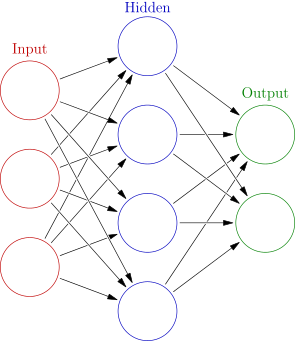
\includegraphics[scale=.5]{imatges/xnn.png}
	\caption{Xarxa neuronal}
\end{figure}
\subsection{Què és una xarxa neuronal?}
Una xarxa neuronal, és una estructura de dades dissenyada per a simular (en la mesura del possible) el comportament del cervell humà. El disseny d'aquesta estructura es fonamenta en diferents capes de neurones interconnectades entre elles i que a través d'un procés iteratiu, són capaces d'ajustar-se i d'aquesta manera adquirir coneixement.
\\\\Una xarxa neuronal està composta per capes de neurones, on sempre hi ha una única capa de neurones d'entrada\footnote{Aquestes neurones d'entrada representen les variables independents sobre les quals es vol fer l'anàlisi (variables explicatives).}, $n$ capes de neurones internes (el nombre de capes depèn de la complexitat del problema a resoldre) i una capa de neurones de sortida.
\begin{itemize}
	\item \textbf{Neurones de la capa d'entrada:} emulen sensors que perceben la informació que es vol processar (variables explicatives).
	\item \textbf{Neurones de les capes internes:} són les neurones que adquireixen el coneixement.
	\item \textbf{Neurones de la capa de sortida:} són les neurones que proporcionen els resultats obtinguts (variables a explicar).
\end{itemize}


%%%%%%%%%%%%%%%%%%%%%%NEURONA%%%%%%%%%%%%%%%%%%%%%%%%
\clearpage
\subsection{Què és una neurona?}
Les neurones són els blocs bàsics en què es recolzen les xarxes neuronals. La seva funcionalitat treballant de forma individual no serveix de gaire, però si que serveix quan treballen de forma estructurada grans quantitats d'aquestes.
\begin{figure}[h!]
	\centering
	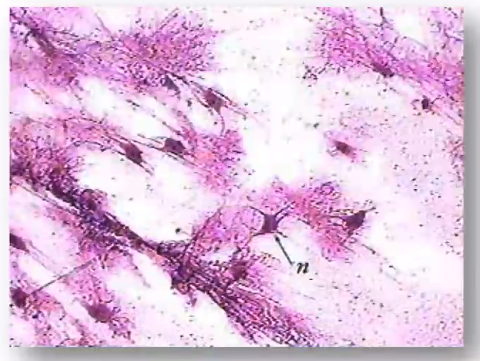
\includegraphics[scale=0.4]{imatges/neurona/1real.png}
	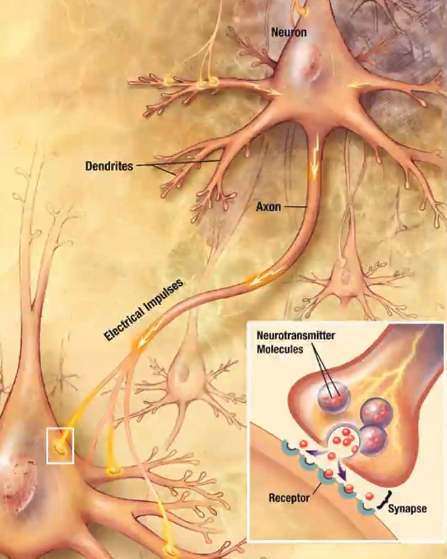
\includegraphics[scale=0.4]{imatges/neurona/3estructura.png}
	\caption{Anatomia d'una neurona real.}
\end{figure}
\\\\Una neurona es compon principalment de:
\begin{itemize}
	\item Núcli.
	\item Dendrites (emissor).
	\item Axó (receptor).
\end{itemize}
La interconnexió de les neurones, es fa a través de l'enviament i recepció d'impulsos elèctrics (\textit{synapses}).
\pagebreak
\clearpage
\begin{figure}[h!]
	\centering
	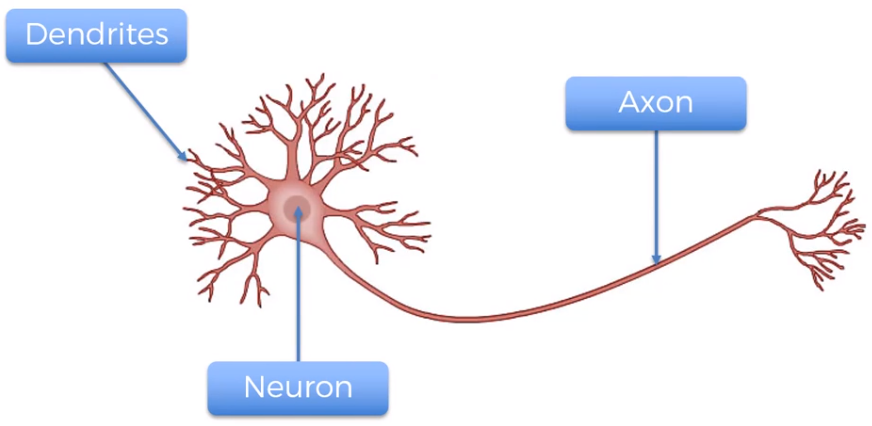
\includegraphics[scale=0.4]{imatges/neurona/9parts.png}
	\caption{Parts d'una neurona.}
\end{figure}
Una xarxa neuronal es pot representar a través d'una caixa negre on hi ha un conjunt d'entrades (neurones d'entrada) i una o vàries sortides (neurones de sortida). Dins d'aquesta caixa, hi han diverses capes de neurones interconnectades que amaguen la complexitat de l'estructura.
\begin{figure}[h!]
	\centering
	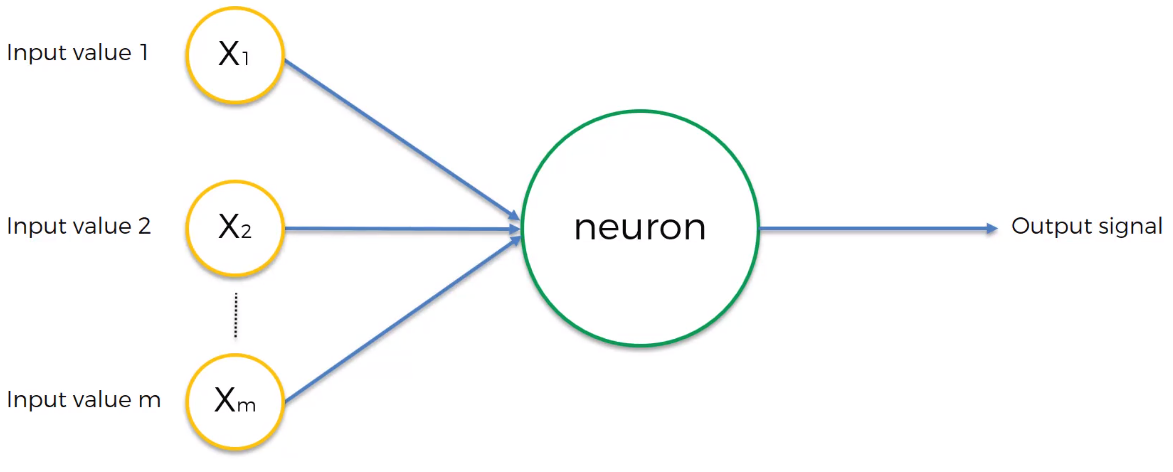
\includegraphics[scale=0.2]{imatges/neurona/5estructura.png}
	\caption{Xarxa neuronal simple (Perceptró).}
\end{figure}
\\\\Les neurones tenen la capacitat d'aprendre, això s'aconsegueix gràcies als pesos (\textit{weights}) assignats a les connexions entre neurones, que determinen el grau d'importància que té cada una de les neurones de la capa anterior. Aquests valors s'actualitzen a través de la tècnica del \textbf{\textit{backpropagation}} (secció \ref{bp}) que utilitza el mètode matemàtic del \textbf{descens del gradient} (secció \ref{dg} i \ref{dge}). 
\\\\La configuració de la xarxa neuronal, determinarà el grau de qualitat de la pròpia xarxa.
\begin{figure}[h!]
	\centering
	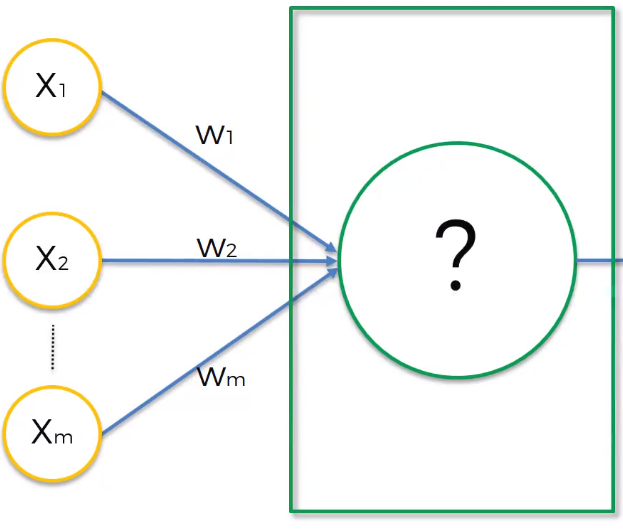
\includegraphics[scale=0.2]{imatges/neurona/6pes.png}
	\caption{Pes (\textit{weights}) de les connexions entre neurones.}
\end{figure}
\\\\A partir dels valors que rep una neurona de la resta, cal generar un valor que serà la sortida, per això s'ha de fer una agregació de valors a través d'una \textbf{funció d'activació} (secció \ref{fa}) que determinarà el grau d'excitació d'aquesta.
\begin{figure}[h!]
	\centering
	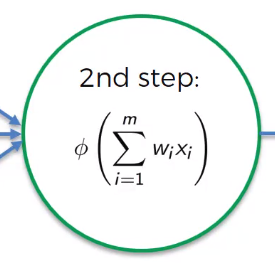
\includegraphics[scale=0.4]{imatges/neurona/7activacio.png}
	\caption{Agregació de valors d'entrada (funció d'activació).}
\end{figure}
\\\\Descrits els diferents components d'una neurona, la integració d'aquesta dins d'una xarxa es pot representar a través de la següent imatge.
\pagebreak
\begin{figure}[h!]
	\centering
	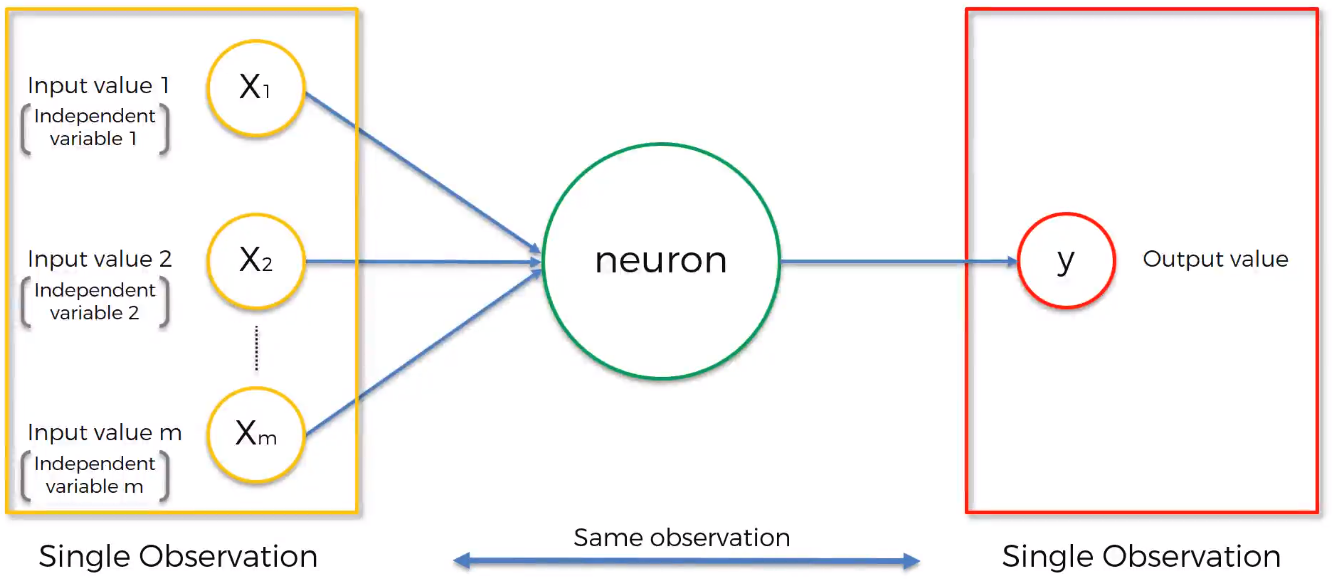
\includegraphics[scale=0.3]{imatges/neurona/8completa.png}
	\caption{Integració d'una neurona en una xarxa neuronal.}
\end{figure}
\\\\S'ha de tenir en compte que el procés d'aprenentatge d'una xarxa neuronal és iteratiu, que tots els valors de les neurones d'entrada corresponen a una mateixa observació, i el valor de sortida al resultat d'aquesta observació.



\clearpage
%%%%%%%%%%%%%%%%%%%%%%FUNCIÓ D'ACTIVACIÓ%%%%%%%%%%%%%%%%%%%%%%%%
\subsection{La funció d'activació \label{fa}}
Les funcions d'activació serveixen per calcular el valor que emetrà una neurona com a sortida. Les funcions d'activació més típics són:
\begin{itemize}
	\item \textit{Threshold function}.
	\item \textit{Sigmoid}.
	\item \textit{Rectifier function}.
	\item \textit{Hyperbolic tangent} (tanh).
\end{itemize}
\subsubsection{\textit{Threshold function}}
El rang de possibles valors per aquesta funció és 0 o 1, això fa que sigui una funció molt rígida i que s'adapti perfectament a casos on es vol una sortida binaria.
\begin{figure}[h!]
	\centering
	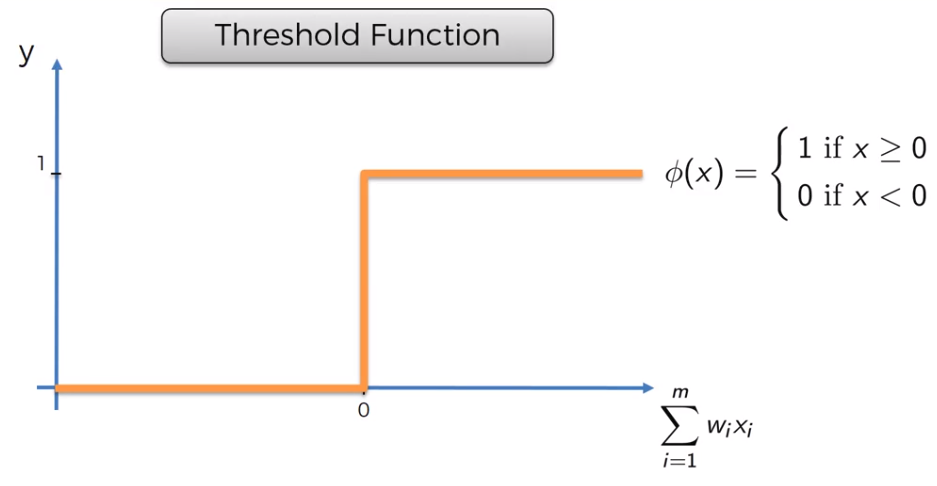
\includegraphics[scale=0.3]{imatges/fa/1threshold.png}
	\caption{\textit{Threshold function.}}
\end{figure}

\subsubsection{\textit{Sigmoid}}
El rang de valors per aquesta funció va de (0, 1) i es sol utilitzar molt com a funció d'activació en l'última capa de neurones, per calcular probabilitats.
\begin{figure}[h!]
	\centering
	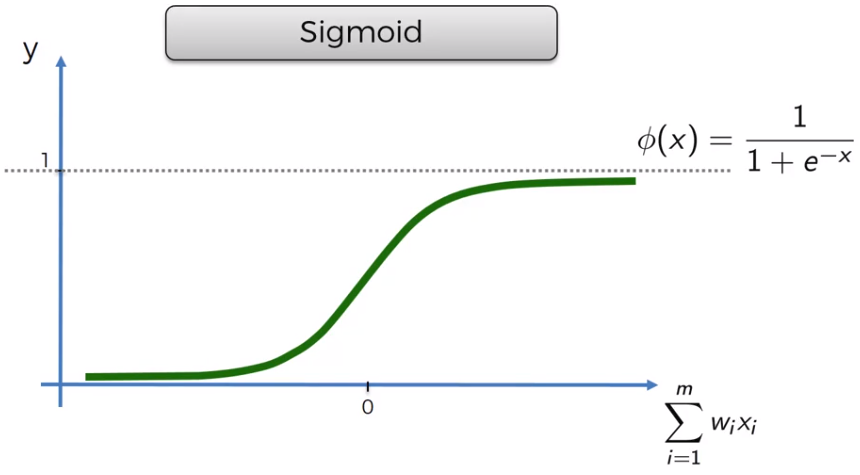
\includegraphics[scale=0.3]{imatges/fa/2sigmoid.png}
	\caption{\textit{Sigmoid function.}}
\end{figure}
\pagebreak
\\\\\\És una funció que s'utilitza molt en la regressió logística.

\subsubsection{\textit{Rectifier function}}
El rang d'aquesta funció va de [0, $x$], on $x$ correspon a la suma ponderada dels valors d'entrada de la capa de neurones anterior.
\begin{figure}[h!]
	\centering
	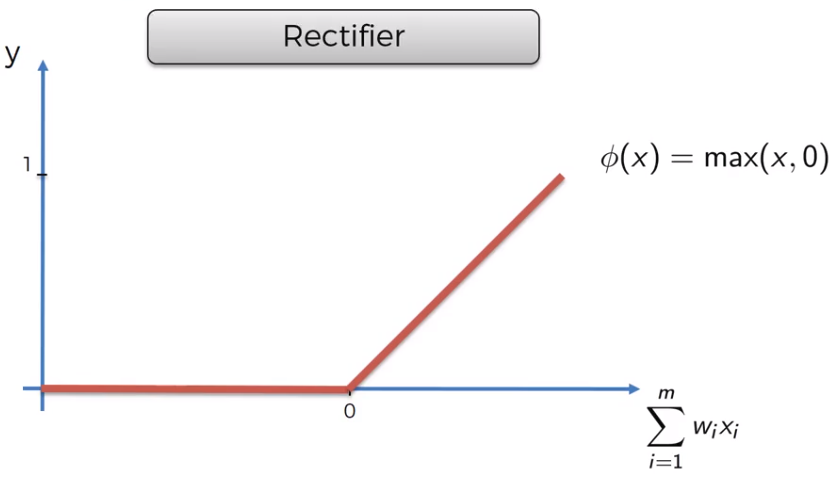
\includegraphics[scale=0.3]{imatges/fa/3rectifier.png}
	\caption{\textit{Rectifier function.}}
\end{figure}

\subsubsection{\textit{Hyperbolic tangent}}
El rang d'aquesta funció va de (-1, 1) i és molt similar a la funció \textit{sigmoid}.
\begin{figure}[h!]
	\centering
	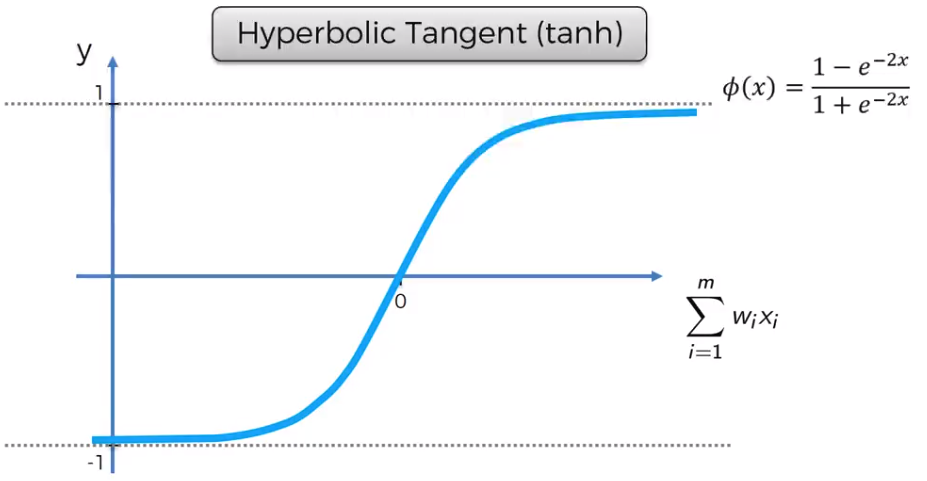
\includegraphics[scale=0.3]{imatges/fa/4tanh.png}
	\caption{\textit{Hyperbolic tangent.}}
\end{figure}

\subsection{Funcions d'activació sobre una xarxa neuronal}
\textbf{Per a cada neurona interna, s'ha de definir una funció d'activació}, per això es poden seguir diferents tècniques.
\begin{itemize}
	\item Assignar una \textbf{mateixa funció d'activació a tota la xarxa neuronal} (rígid però senzill de desenvolupar i mantenir).
	\item Assignar una \textbf{mateixa funció d'activació a nivell de capa de neurones}.
	\item Assignar una \textbf{funció d'activació diferent per a cada neurona} (complex però potent).
\end{itemize}
La tècnica a utilitzar dependrà sempre del tipus de problema a resoldre, de la seva complexitat i de la potencia disponible.
\begin{figure}[h!]
	\centering
	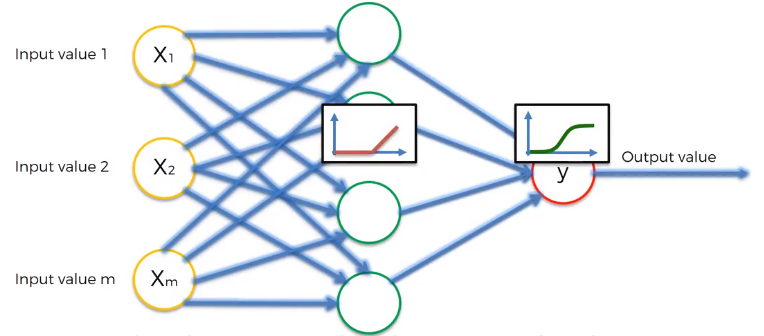
\includegraphics[scale=0.3]{imatges/fa/5complet.png}
	\caption{Aplicació de funcions d'activació sobre una xarxa neuronal.}
\end{figure}



\clearpage
%%%%%%%%%%%%%%%%%%%%%%COM FUNCIONEN?%%%%%%%%%%%%%%%%%%%%%%%%
\subsection{Com funcionen?}
El funcionament de les xarxes neuronals es basa en la configuració que s'ha de fer sobre les capes de neurones internes. 
\\\\Per veure millor com funcionen, s'utilitzarà un exemple d'una possible aplicació real, en la que es disposa d'un conjunt dades en base a diferents habitatges que tenen els següents paràmetres:
\begin{itemize}
	\item Dimensions.
	\item Nombre de lavabos.
	\item Distància del centre de la ciutat.
	\item Antiguitat.
\end{itemize}

Sobre aquestes dades, es vol \textbf{especular el preu} que pot tenir un habitatge en base a les seves propietats.
\\\\A nivell de neurona, s'ha d'elegir quins paràmetres actuen sobre el seu càlcul i crear una connexió que enllaçi les neurones. 
\\\\En aquests exemple, la primera neurona s'utilitza per influir en l'especulació del preu d'acord amb les mides de l'habitatge i la distància que està del centre de la ciutat. 
\\\\De forma intuïtiva es pot pensar que els habitatges més grans i que estan properes al centre de la ciutat són més cars, i per això, la primera neurona interna influirà en el preu en base aquests dos paràmetres.
\begin{figure}[h!]
	\centering
	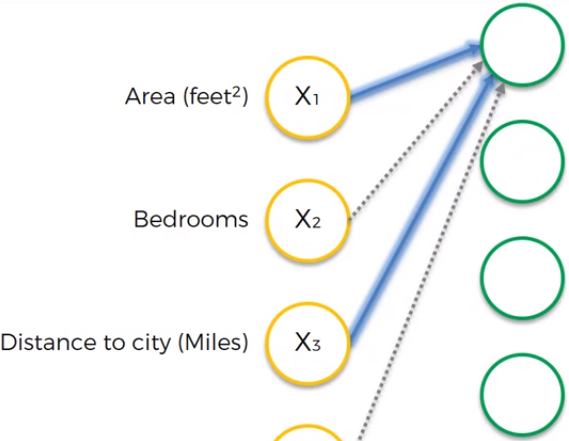
\includegraphics[scale=0.3]{imatges/funcionament/1basic.png}
	\caption{Configuració d'una neurona.}
\end{figure}
\pagebreak
\\\\D'aquesta manera, una possible configuració completa d'una xarxa molt senzilla per calcular el preu pot ser com en la següent imatge.
\begin{figure}[h!]
	\centering
	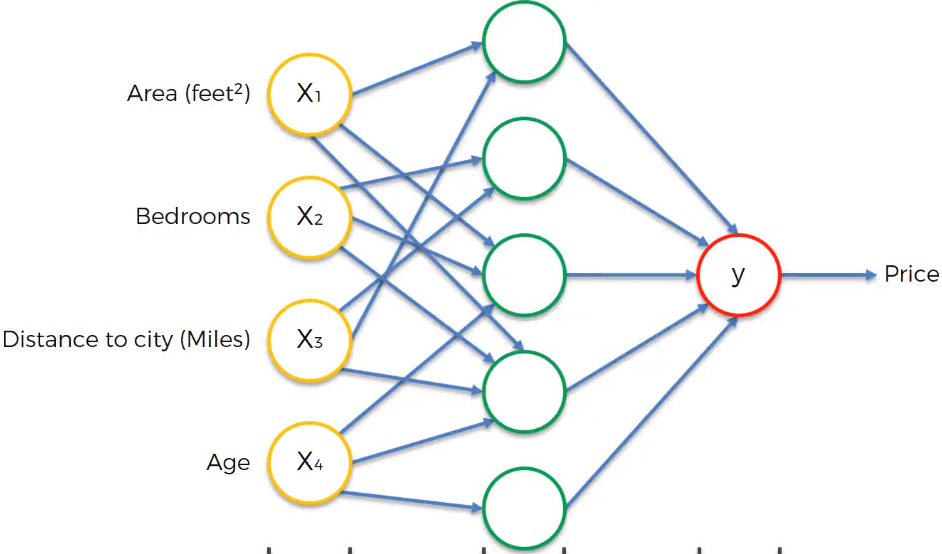
\includegraphics[scale=0.3]{imatges/funcionament/2completa.png}
	\caption{Configuració completa d'una xarxa neuronal senzilla.}
\end{figure}
\\\\Les neurones que no tenen impacte en el càlcul no es representen utilitzant connexions, això es pot interpretar com que tenen un impacte nul sobre aquell càlcul.

\clearpage
%%%%%%%%%%%%%%%%%%%%%%COM APRENEN?%%%%%%%%%%%%%%%%%%%%%%%%
\subsection{Com aprenen?}
Com ja s'ha dit anteriorment, les xarxes neuronals es basen en un mecanisme d'aprenentatge iteratiu amb el qual van adquirint coneixement a mesura que guanyen experiència. Per aquest motiu, és necessari dividir les etapes de funcionament d'una xarxa neuronal en:
\begin{itemize}
	\item \textbf{Etapa d'entrenament:} en aquesta etapa es proporcionen multiples exemples a partir dels quals s'adquireix la gran majoria del coneixement. S'ha de tenir en compte que durant aquest procés cal saber el resultat correcte per obtenir una xarxa ben entrenada.
	\item \textbf{Etapa de test:} en aquesta etapa es posa a prova la xarxa, proporcionant noves dades i analitzant els resultats. En cas de comptar amb el resultat correcte per aquestes dades, la xarxa pot continuar aprenent.
\end{itemize}
Durant l'etapa d'entrenament i un cop s'obté el resultat proporcionat de la xarxa, cal comprar-lo amb el resultat real i extreure un valor que representi la distància que hi ha entre el valor preedit i el correcte. Aquesta magnitut s'extreu a partir de la funció de cost. 
\begin{figure}[h!]
	\centering
	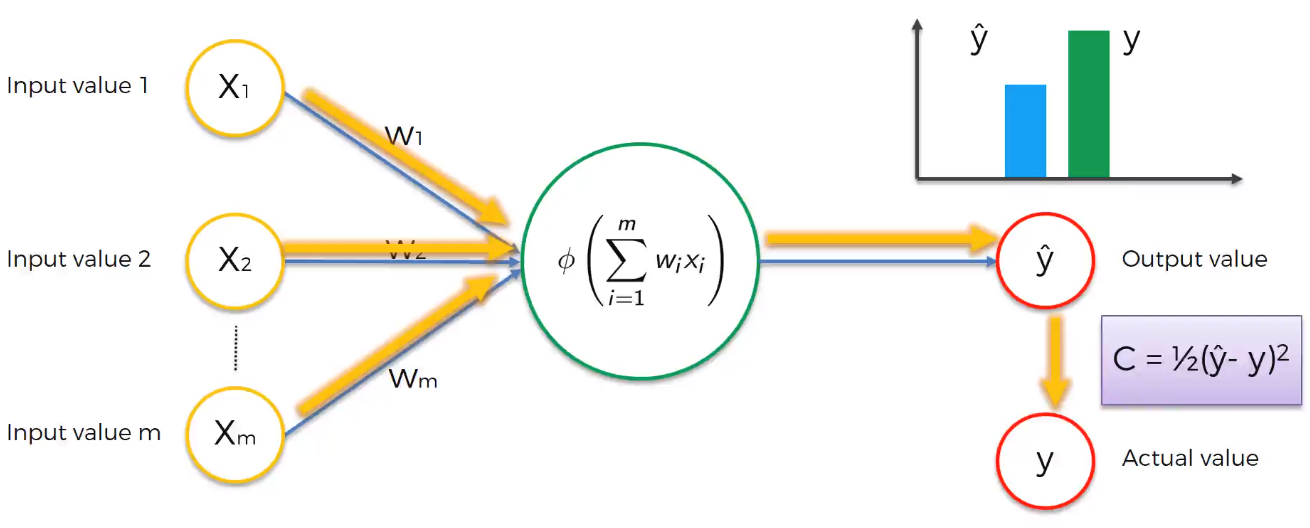
\includegraphics[scale=0.3]{imatges/aprendre/1aprendre.png}
	\caption{Funció de cost.}
\end{figure}
El valor proporcionat per la funció de cost, s'utilitza com entrada del mecanisme d'adaptació d'adaptació de la xarxa(\textit{backpropagation}).
\begin{figure}[h!]
	\centering
	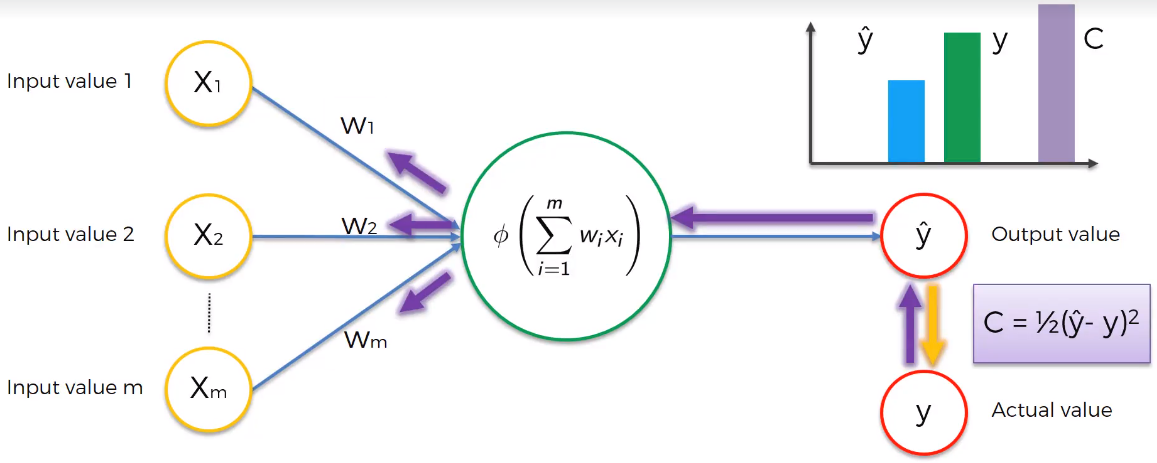
\includegraphics[scale=0.3]{imatges/aprendre/2bp.png}
	\caption{\textit{Backpropagation}.}
\end{figure}
\\\\Un possible exemple seria l'utilització d'una xarxa neuronal per a desenvolupar una regressió que calculés una aproximació de la nota a treure en un examen en base a:
\begin{itemize}
	\item Nombre d'hores empreades a estudiar.
	\item Nombre d'hores dormides.
	\item Última nota obtinguda en el test.
\end{itemize}
L'etapa d'aprenentatge per aquest problema i donada una xarxa neuronal molt sencilla queda il·lustrada en la següent imatge.
\begin{figure}[h!]
	\centering
	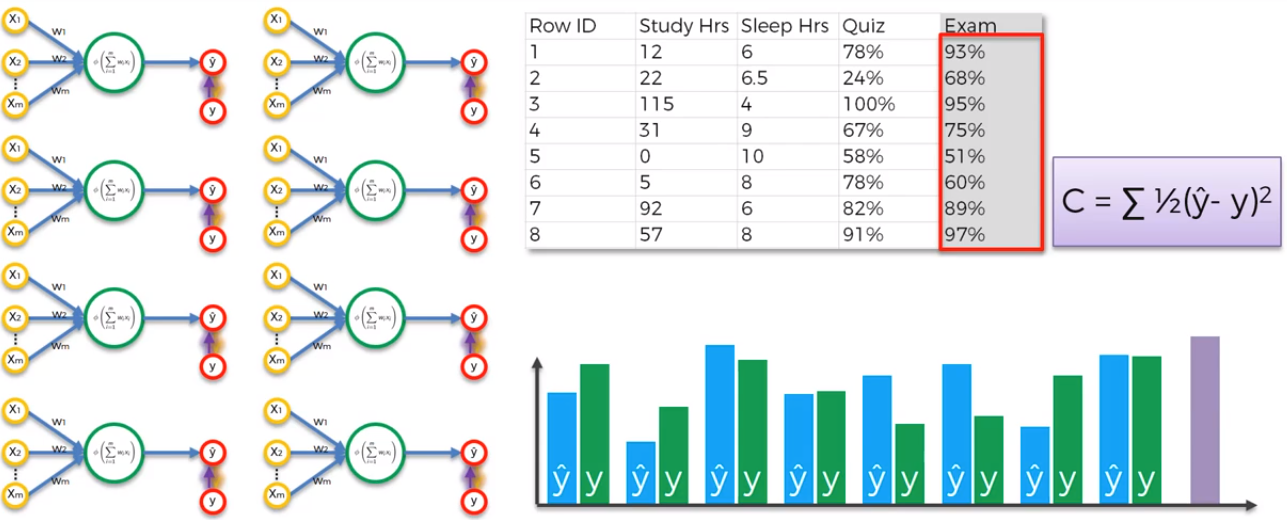
\includegraphics[scale=0.3]{imatges/aprendre/3aprendre.png}
	\caption{Etapa de càlcul.}
	\label{fig:3aprendre}
\end{figure}
\\\\Un cop obtingut els resultats de la xarxa, s'ha d'aplicar la funció de cost que compara el valor preedit amb el valor obtingut realment i amb aquest resultat aplicar la tècnica de \textit{backpropagation} com es mostra en la següent imatge.
\begin{figure}[h!]
	\centering
	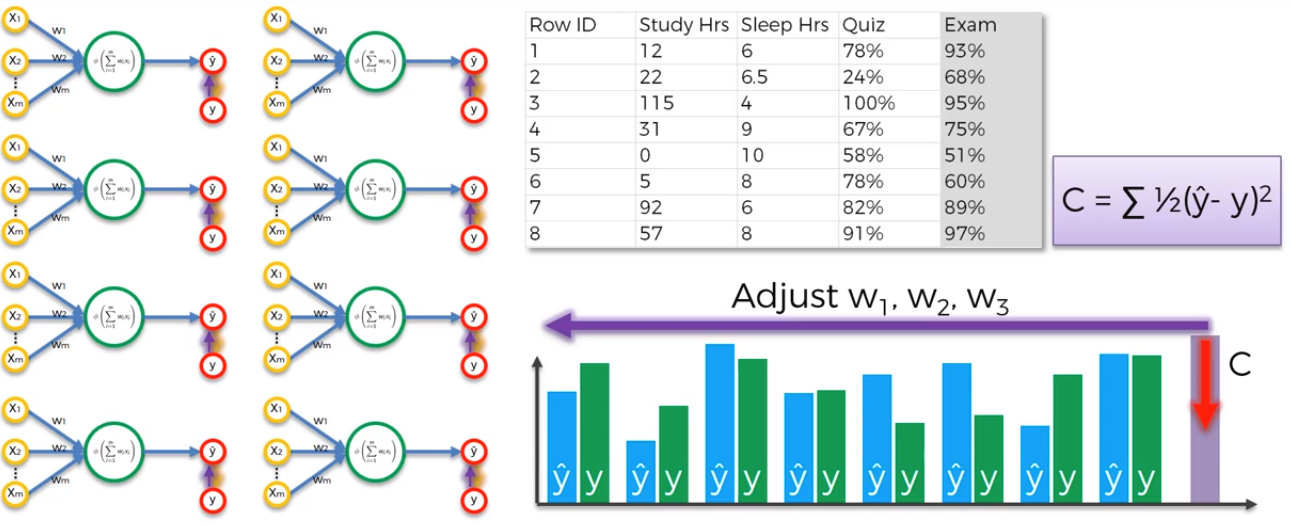
\includegraphics[scale=0.3]{imatges/aprendre/4bp.png}
	\caption{Etapa d'aprenentatge.}
	\label{fig:4bp}
\end{figure}
\\\\És important veure que en la figura \ref{fig:3aprendre} i \ref{fig:4bp} s'esta utilitzant la mateixa xarxa neuronal però utilitzant diferents dades, i que la funció de cost per aplicar el \textit{backpropagation} utilitza tots els valors disponibles en el conjunt d'entrenament. \footnote{Una iteració sobre totes les dades d'entrenament es coneix com un \textit{epoch}.}

\clearpage
%%%%%%%%%%%%%%%%%%%%%%DESCENS DEL GRADIENT%%%%%%%%%%%%%%%%%%%%%%%%
\subsection{Descens del gradient\label{dg}}
Per aconseguir que la xarxa neuronal aprengui, cal modificar els pessos de les synapses que connecten les diferents capes de neurones.
\\\\Donat una xarxa neuronal simple on hi ha 4 neurones en la capa d'entrada, 5 neurones en la capa interna i 1 neurona en la capa de sortida, tenim un total de 5 possibles synapses. 
\begin{figure}[h!]
	\centering
	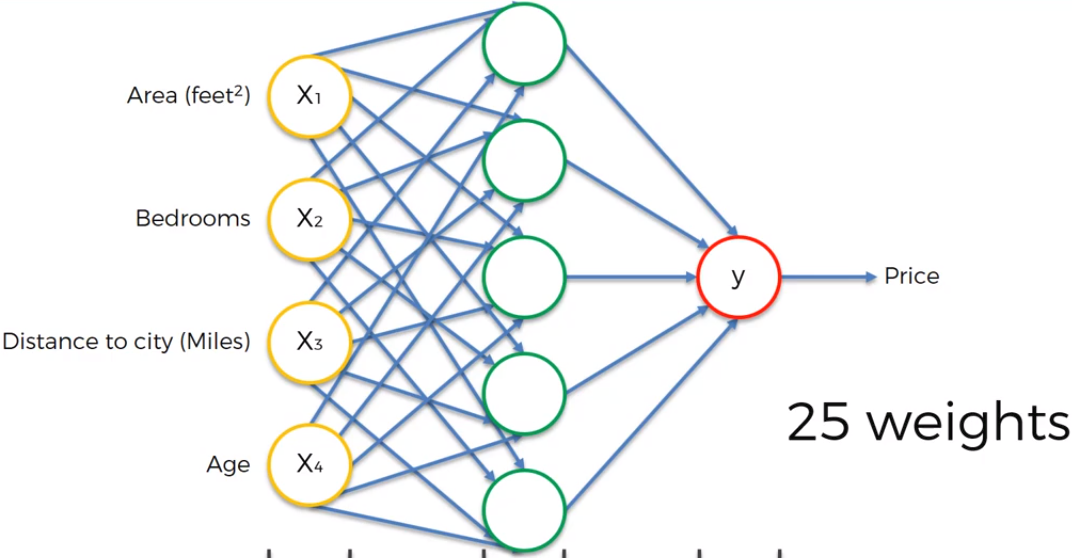
\includegraphics[scale=0.3]{imatges/dg/1dg.png}
	\caption{Etapa d'aprenentatge.}
	\label{fig:4bp}
\end{figure}
\\\\Ara assumim que les variables d'entrada tenen un rang de possibles valors que va de [1, 1000] i volem ajustar el coneixement modificant aleatoriament els 25 possibles pesos, això fa que hi hagui $1000^{25}$ possibles combinacions. Tenint en compte que el supercomputador més potent a nivell mundial \textit{sunway taihulight} té una potència de calcul d'aproximadament 93 PFLOPs.\footnote{Pot arribar a executar aproximadament $9.3 \cdot 10^{15}$ operacions cada segon.}
\pagebreak
\begin{figure}[h!]
	\centering
	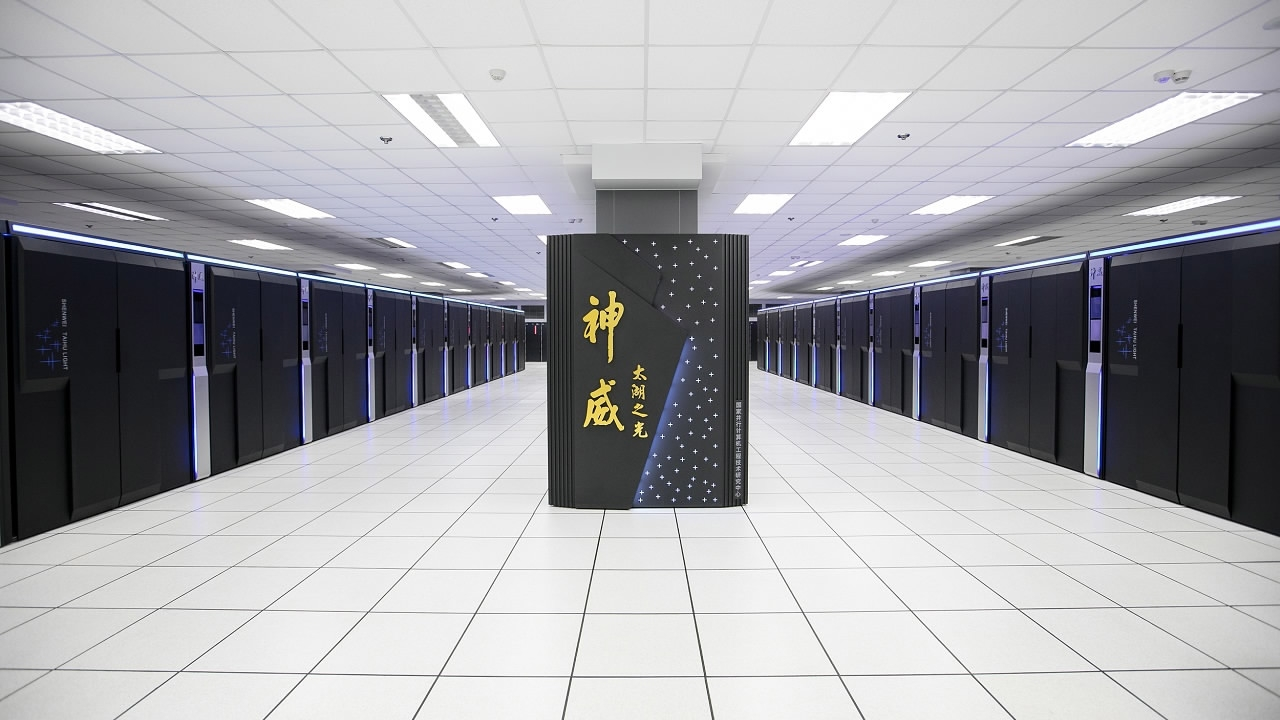
\includegraphics[scale=0.3]{imatges/dg/sunlight.jpg}
	\caption{Sunway taihulight.}
\end{figure}
\\\\Caldrien $1.08 \cdot 10^{58}$ segons, és a dir $3.42 \cdot 10^{50}$ anys. 
$$\frac{1000^{25}}{93 \cdot 10^{15}} \approx 1.08 \cdot 10^{58} segons \approx 3.42 \cdot 10^{50} anys$$ 
Tot això tenint en compte que es pot fer una assignació de pesos per operació, cosa que no pot ser com ja hem vist abans. 
\\\\I si tenim una xarxa més complexa?
\begin{figure}[h!]
	\centering
	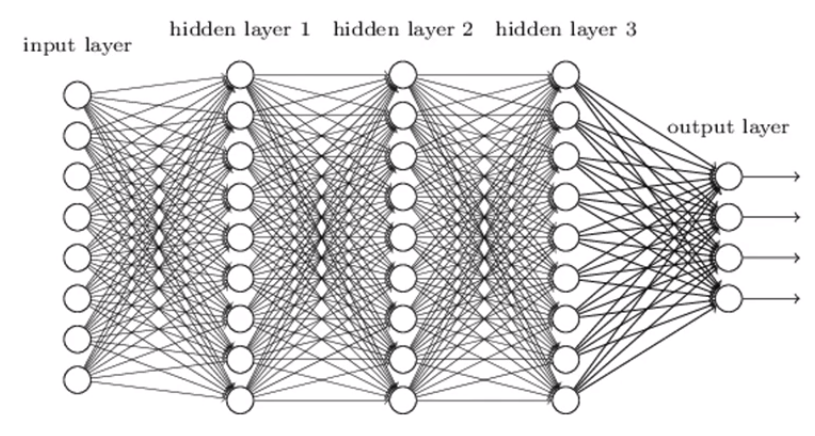
\includegraphics[scale=0.25]{imatges/dg/xnComplexa.png}
	\caption{Xarxa neuronal complexa.}
\end{figure}
\\\\Vist que utilitzar força bruta no serveix en aquest problema cal utilitzar una altre mètode i en aquest cas el descens del gradient.
\\\\El descens del gradient és el mètode matemàtic en que es basa la tècnica \textit{backpropagation} per aconseguir absorbir el coneixement adquirit durant la fase d'entrenament. 
\\\\Aquesta tècnica radica en buscar el camí més curt per reduir la funció de cost, això es fa a través de la derivada de la funció de cost que determina la pendent en un punt donat.
\begin{figure}[h!]
	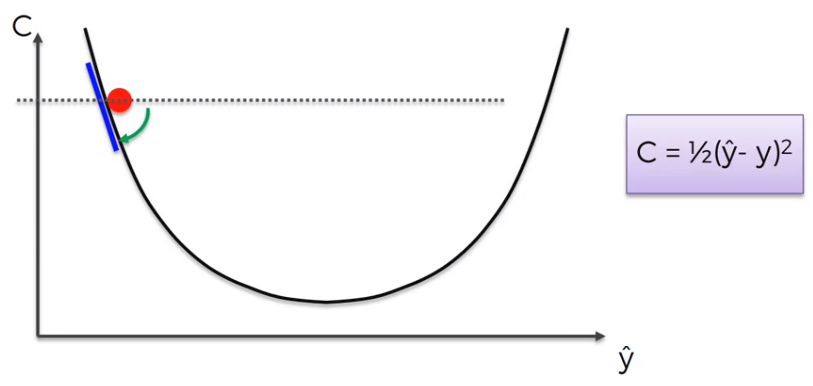
\includegraphics[scale=0.25]{imatges/dg/2dg2.png}
	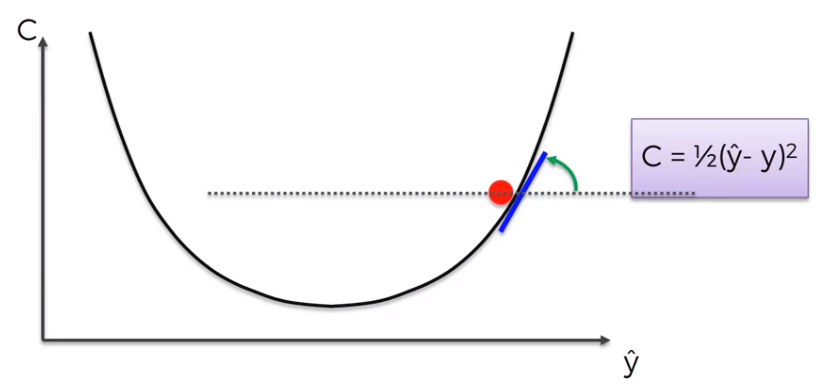
\includegraphics[scale=0.25]{imatges/dg/3dg3.png}
	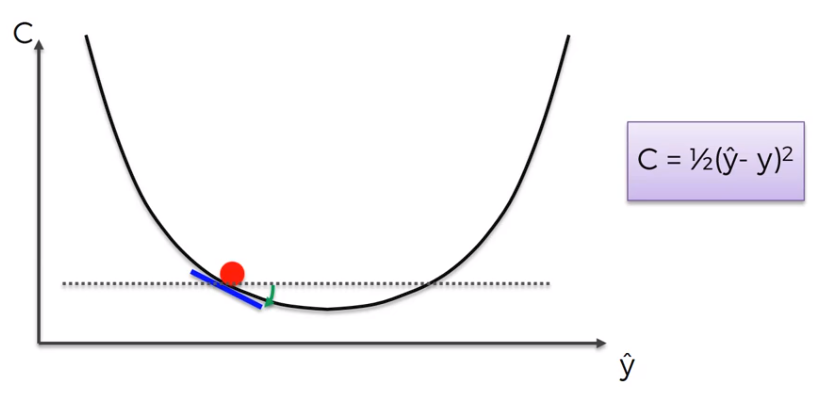
\includegraphics[scale=0.25]{imatges/dg/4dg4.png}
	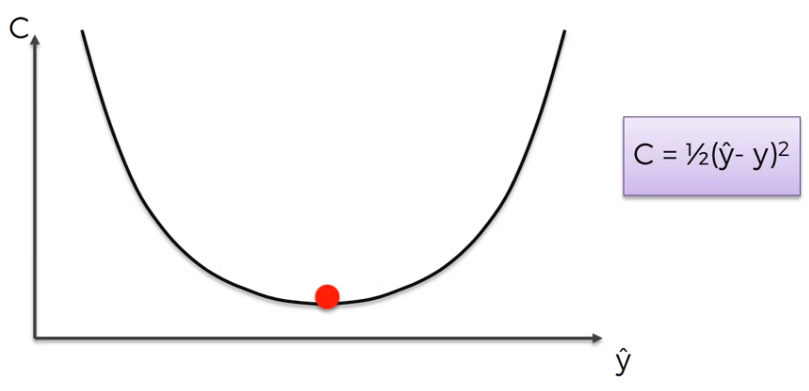
\includegraphics[scale=0.25]{imatges/dg/5dg5.png}
	\caption{Descens del gradient.}
\end{figure}
\\\\Així doncs, utilitzant la tècnica del descens del gradient i per aquesta funció de cost, podem trobar l'òptim en pocs passos (quatre passos en aquest cas).
\begin{figure}[h!]
	\centering
	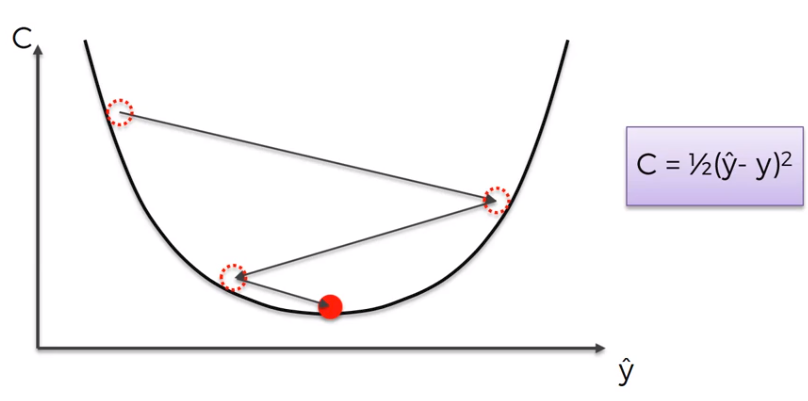
\includegraphics[scale=0.3]{imatges/dg/6dg6.png}
	\caption{Descens del gradient.}
\end{figure}
\pagebreak 
\\\\Les següents imatges mostren el procés del descens del gradient tenint en compte diferents dimensions.
\begin{figure}[h!]
	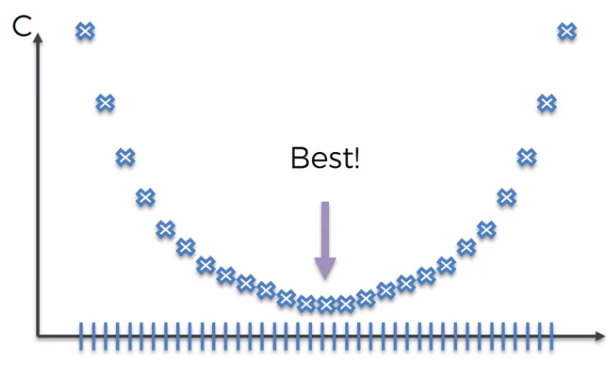
\includegraphics[scale=0.25]{imatges/dg/dg1d.png}
	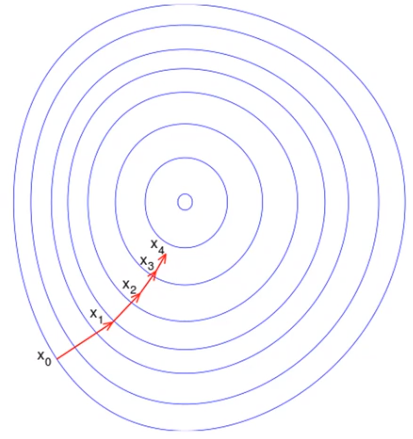
\includegraphics[scale=0.25]{imatges/dg/dg2d.png}
	\centering
	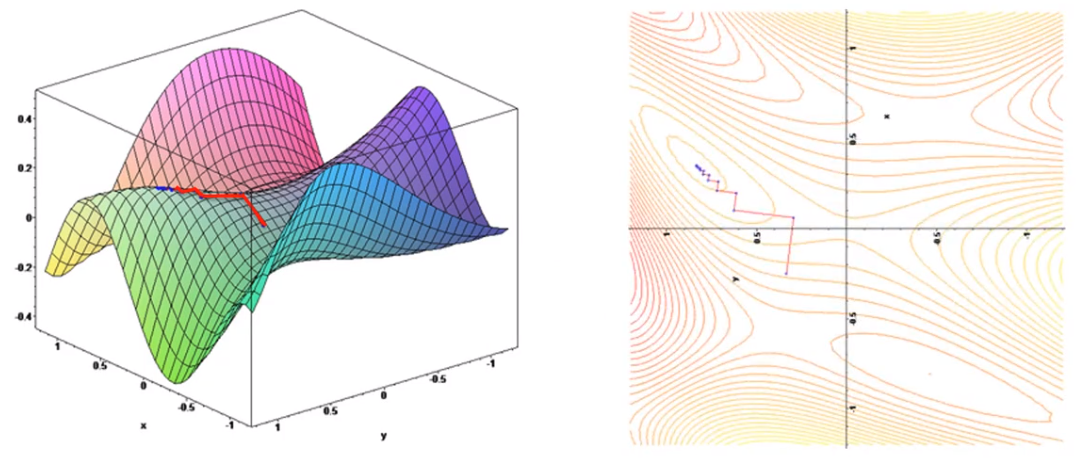
\includegraphics[scale=0.4]{imatges/dg/dg3d.png}
	\caption{Descens del gradient en diferents dimensions.}
\end{figure}

\clearpage
%%%%%%%%%%%%%%%%%%%%%%DESCENS DEL GRADIENT ESTOCÀSTIC%%%%%%%%%%%%%%%%%%%%%%%%
\subsection{Descens del gradient estocàstic\label{dge}}
El típic problema que podem trobar a l'hora d'utilitzar el mètode del descens del gradient\footnote{Notar que aquest problema no es tindrà si la funció és convexa.}, és el de no arribar a trobar l'òptim global a causa de que s'ha arribat a un òptim local. Això vol dir que no arribem a entrenar la xarxa tant com voldriem. Per resoldre aquest problema es pot utilitzar el mètode del descens del gradient estocastic.
\begin{figure}[h!]
	\centering
	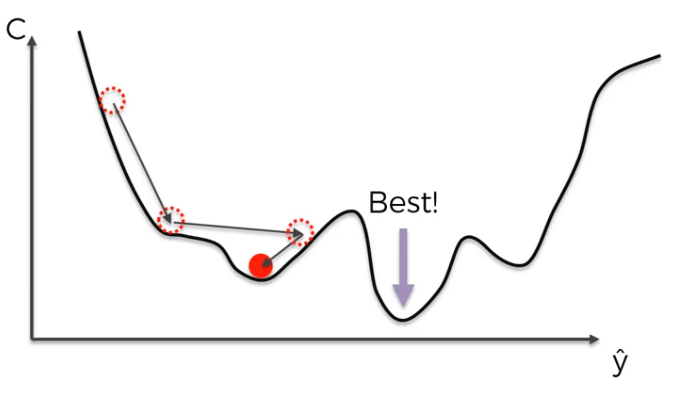
\includegraphics[scale=0.4]{imatges/dge/1dge.png}
	\caption{Òptim local.}
\end{figure}
\\\\El descens del gradient estocàstic s'aconsegueix aplicant la funció de \textit{backpropagation} per cada registre processat per la xarxa, d'aquesta manera s'obté una major fluctuació i així hi ha més probabilitat de no caure en un òptim local.
\pagebreak
\begin{figure}[h!]
	\centering
	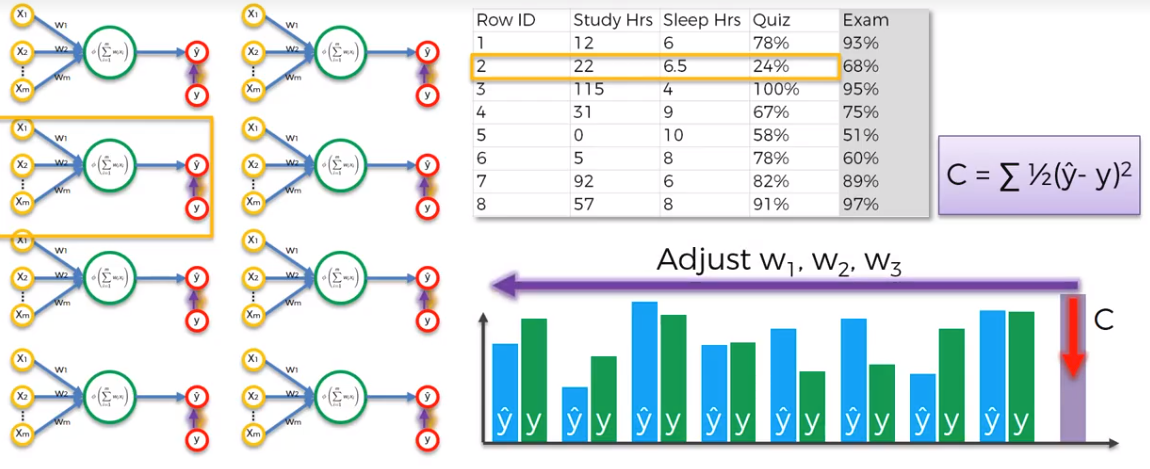
\includegraphics[scale=0.4]{imatges/dge/2dge.png}
	\caption{Descens del gradient estocàstic.}
\end{figure}
\\\\És important veure que aquest mètode és indeterminista ja que el resultat dependrà de l'ordre en que es processin els registres.


\clearpage
%%%%%%%%%%%%%%%%%%%%%%BACKPROPAGATION%%%%%%%%%%%%%%%%%%%%%%%%
\subsection{Backpropagation\label{bp}}
El Backpropagation és un algorisme complex a nivell matemàtic que permet ajustar tots els pesos a l'hora, es a dir, permet identificar quins són els pesos que estan causant més error i en quina mesura s'han de modificar.
\\\\Durant l'entrenament d'una xarxa neuronal, podem destacar dues fases.
\\\\La fase de \textit{Forwardpropagation} on entren valors per les neurones d'entrada i es genera un resultat.
\begin{figure}[h!]
	\centering
	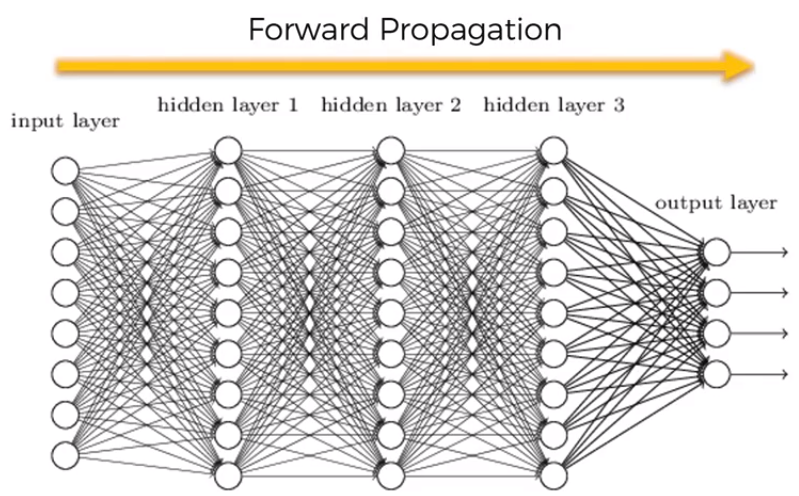
\includegraphics[scale=0.25]{imatges/bp/1bp.png}
	\caption{Forwardpropagation.}
\end{figure}
\\\\La fase de \textit{Backpropagation} on es calcula l'error comés amb el resultat i s'intenten ajustar els pesos de les synapses.
\begin{figure}[h!]
	\centering
	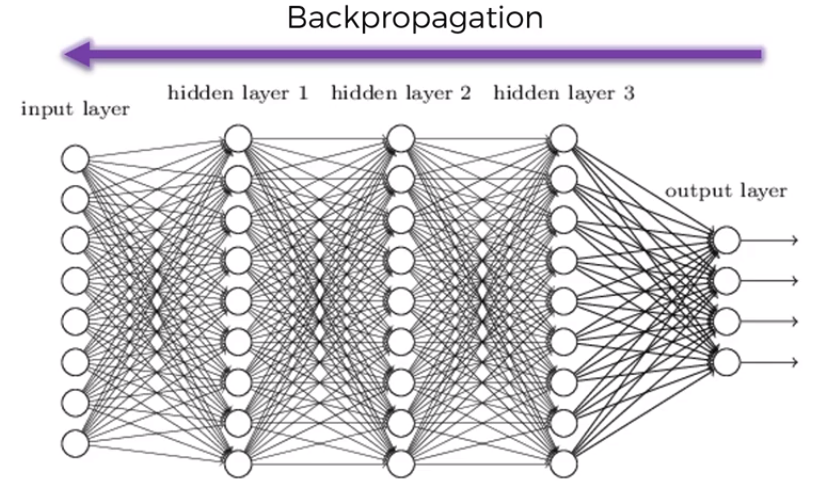
\includegraphics[scale=0.25]{imatges/bp/2bp.png}
	\caption{Backpropagation.}
\end{figure}
\pagebreak
\\\\Els passos que es segueixen durant l'entrenament d'una xarxa són:
\begin{enumerate}
	\item Iniciar aleatoriament (amb un valor pròxim a 0) els pesos de les synapses.
	\item Assignar un valor (de la mateixa observació) a cada una de les neurones de la capa d'entrada.
	\item \textit{Forwardpropagation}, activant les neurones.
	\item Calcular l'error generat a través de la funció de cost.
	\item \textit{Backpropagation}, corregint l'error comés.
	\item Repetir passos 1-5 fins arribar a processar totes les observacions.
	\item S'ha completat una \textit{epoch}, fer més \textit{epochs} repetint passos 1-6.
\end{enumerate}

\clearpage
\section{Classificació utilitzant una xarxa neuronal}
\subsection{Dades\label{dades}}
Les dades amb les que es treballarà (\path{Churn_Modelling.csv}), corresponen a 10.000 clients d'un banc (fictici) amb els següents camps:
\begin{itemize}
	\item \textbf{RowNumber:} identificador de registre [1-10.000].
	\item \textbf{CustomerId:} identificador univoc del client.
	\item \textbf{Surname:} Cognom del client.
	\item \textbf{CreditScore:} Nombre de punts.
	\item \textbf{Geography:} País d'origen.
	\item \textbf{Gender:} Sexe.
	\item \textbf{Age:} Edat.
	\item \textbf{Tenure:} Nombre d'anys des de que és client.
	\item \textbf{Balance:} Ingressos fets respecte les despeses.
	\item \textbf{NumOfProduct:} Nombre de productes del banc que ha adquirit.
	\item \textbf{HasCrCard}: Si té o no targeta de crèdit.
	\item \textbf{IsActiveMember:} Si utilitza algun dels productes amb regularitat.
	\item \textbf{EstimateSalary:} Salari anual estimat.
	\item \textbf{Exited:} Si es preveu que el client abandonarà o no el banc.
\end{itemize}
En la següent imatge es pot veure un extracte dels 10 primers registres del \textit{dataset}.
\pagebreak
\begin{figure}[h!]
	\centering
	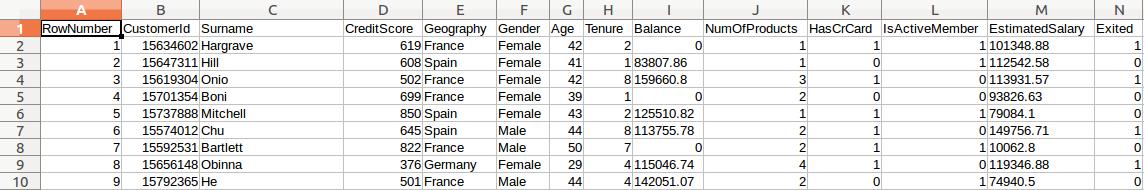
\includegraphics[scale=0.4]{imatges/dades/dades.png}
	\caption{Dades.}
\end{figure}

\clearpage
\subsection{Problema}
A partir de les dades descrites en la secció \ref{dades}, volem arribar a respondre la següent pregunta mitjançant classificació utilitzant una xarxa neuronal.
\begin{center}
\textbf{Es preveu que en un perïode de 6 mesos, el client abandoni el banc?}
\end{center}
La resposta correcte a aquesta pregunta correspon al valor de l'últim camp \textit{exited}, on:
\begin{itemize}
	\item 0: si no es preveu que el client abandoni el banc.
	\item 1: si es preveu que el client abandoni el banc.
\end{itemize}

\clearpage
\subsection{Eines a utilitzar}
Per desenvolupar aquest programa s'utilitzaràn les següents eines.
\begin{itemize}
	\item \textit{Python:} Com a llenguatge de programació (a nivell d'exemple), s'ha decidit utilitzar python, el codi complet es pot consultar en l'annex \ref{app:python}.
	\begin{center}
		
\includegraphics[width=3cm]{imatges/eines/python.png}
	\end{center}
	
	\item \textit{R:} També s'ha desenvolupat la xarxa neuronal utilitzant el llenguatge de programació R (per completitud del projecte), el codi es pot consultar en l'annex (app:r).
	\begin{center}
		
\includegraphics[width=3cm]{imatges/eines/r.png}
	\end{center}	
	
	\item \textit{Theano:} Llibreria de computació numèrica de codi obert, permet efectuar calculs no només sobre la \textit{CPU} sinó que també sobre la \textit{GPU}.
	\begin{center}
		
\includegraphics[scale=0.4]{imatges/eines/theano.png}
	\end{center}
	Instal·lació: \path{\$pip install --upgrade --no-deps git+git://github.com/Theano/Theano.git}	
	
	\item \textit{Tensorflow:} Llibreria de computació numèrica de codi obert, inicialment desenvolupada pel \textit{Google brain team} i actualment alliberada sota la llicència \textit{Apache license 2.0}. 
	\begin{center}
		
\includegraphics[scale=0.4]{imatges/eines/tensorflow.png}
	\end{center}
	Instal·lació: \path{https://www.tensorflow.org/versions/r0.12/get_started/os_setup.html}
	
	\item \textit{Keras:} Llibreria que serveix d'envoltori per les llibreries \textit{Theano} i \textit{Tensorflow}, permetent crear xarxes neuronals amb relativament poques lineas de codi.
	\begin{center}
		
\includegraphics[scale=0.4]{imatges/eines/keras.png}	
	\end{center}
	Instal·lació: \path{\$pip install --upgrade keras}
	
\end{itemize}
S'ha de tenir en compte que les llibreries \textit{Theano} i \textit{Tensorflow} estan orientades al món de la investigació i el densevolupament professional, i per tant, si s'utilitzen s'ha de desenvolupar la xarxa neuronal des de 0 (la qual cosa suposa un gran esforç i un alt nivell de coneixement sobre la materia).
\clearpage
\subsection{Classificació}
Els passos a seguir per aplicar la classificació utilitzant una xarxa neuronal són.
\begin{enumerate}
	\item Preprocessament de les dades.
	\item Creació de la xarxa neuronal.
	\item Classificació.
	\item Evaluar la precissió del model.
\end{enumerate}
\subsubsection{Processament de les dades}
En aquest apartat es mostra el codi necessari per efectuar el processament de dades que s'ha de fer abans d'exectuar la xarxa neuronal.
\lstinputlisting[language=Python]{codi/python/part1.py}

\subsubsection{Creació de la xarxa neuronal}
En aquest apartat es mostra el codi necessari per efectuar la creació de la xarxa neuronal.
\lstinputlisting[language=Python]{codi/python/part2.py}
\begin{figure}[h!]
	\centering
	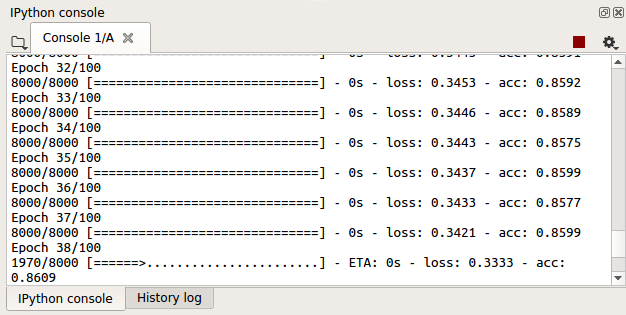
\includegraphics[scale=0.4]{imatges/python/entrenament.png}
	\caption{Entrenament de la xarxa.}
\end{figure}
\pagebreak
És important notar que al final de l'entrenament de la xarxa (en l'últim \textit{poch}) hi ha hagut una \textbf{precissió de 86\%}.

\subsubsection{Classificació}
En aquest apartat es mostra el codi necessari per efectuar la classificació de les dades de test.
\lstinputlisting[language=Python]{codi/python/part3.py}

\pagebreak
\subsubsection{Evaluar la precissió del model}
En aquest apartat es mostra l'efectivitat de la classificació que ha fet la xarxa, comparant les prediccions amb els valors reals.
\lstinputlisting[language=Python]{codi/python/part4.py}
S'ha obtingut una precissió del 86\% aproximadament. En la següent matriu de confusió es pot veure la relació de resultats.
\begin{figure}[h!]
	\centering
	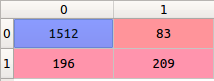
\includegraphics[scale=0.7]{imatges/python/cm.png}
	\caption{Matriu de confusió.}
\end{figure}

%%%%%%%%%%%%%%%BIBLIOGRAFIA%%%%%%%%%%%%%%%%%
\clearpage
\begin{thebibliography}{9}
	\bibitem{ANN}\textit{Xarxa neuronal}:
  	\\\path{https://en.wikipedia.org/wiki/Artificial_neural_network}
	\bibitem{AF1}\textit{Deep sparse rectifier neural networks}:
  	\\\path{http://proceedings.mlr.press/v15/glorot11a/glorot11a.pdf}
	\bibitem{FC}\textit{Funcions de cost més tipiques}:
  	\\\path{https://stats.stackexchange.com/questions/154879/a-list-of-cost-functions-used-in-neural-networks-alongside-applications}
	\bibitem{SC}\textit{Top 500 supercomputers}:
  	\\\path{https://www.top500.org/system/178764}
  	\bibitem{DG}\textit{Descendent del gradient}:
  	\\\path{http://iamtrask.github.io/2015/07/27/python-network-part2/}
  	\bibitem{DGBP}\textit{Descendent del gradient i Backpropagation}:
  	\\\path{http://neuralnetworksanddeeplearning.com/chap2.html}
\end{thebibliography}

\clearpage
\begin{appendices}
\section{Codi}
\subsection{Python}
\lstinputlisting[language=Python]{codi/python/complet.py}
\clearpage
\subsection{R}
\lstinputlisting[language=R]{codi/R/complet.R}
\end{appendices}
\end{document}